\section{Evaluation}
\label{sec-evaluation}

\XXXnote{GWA: TODO: Integrate.}

\begin{figure}
\centering
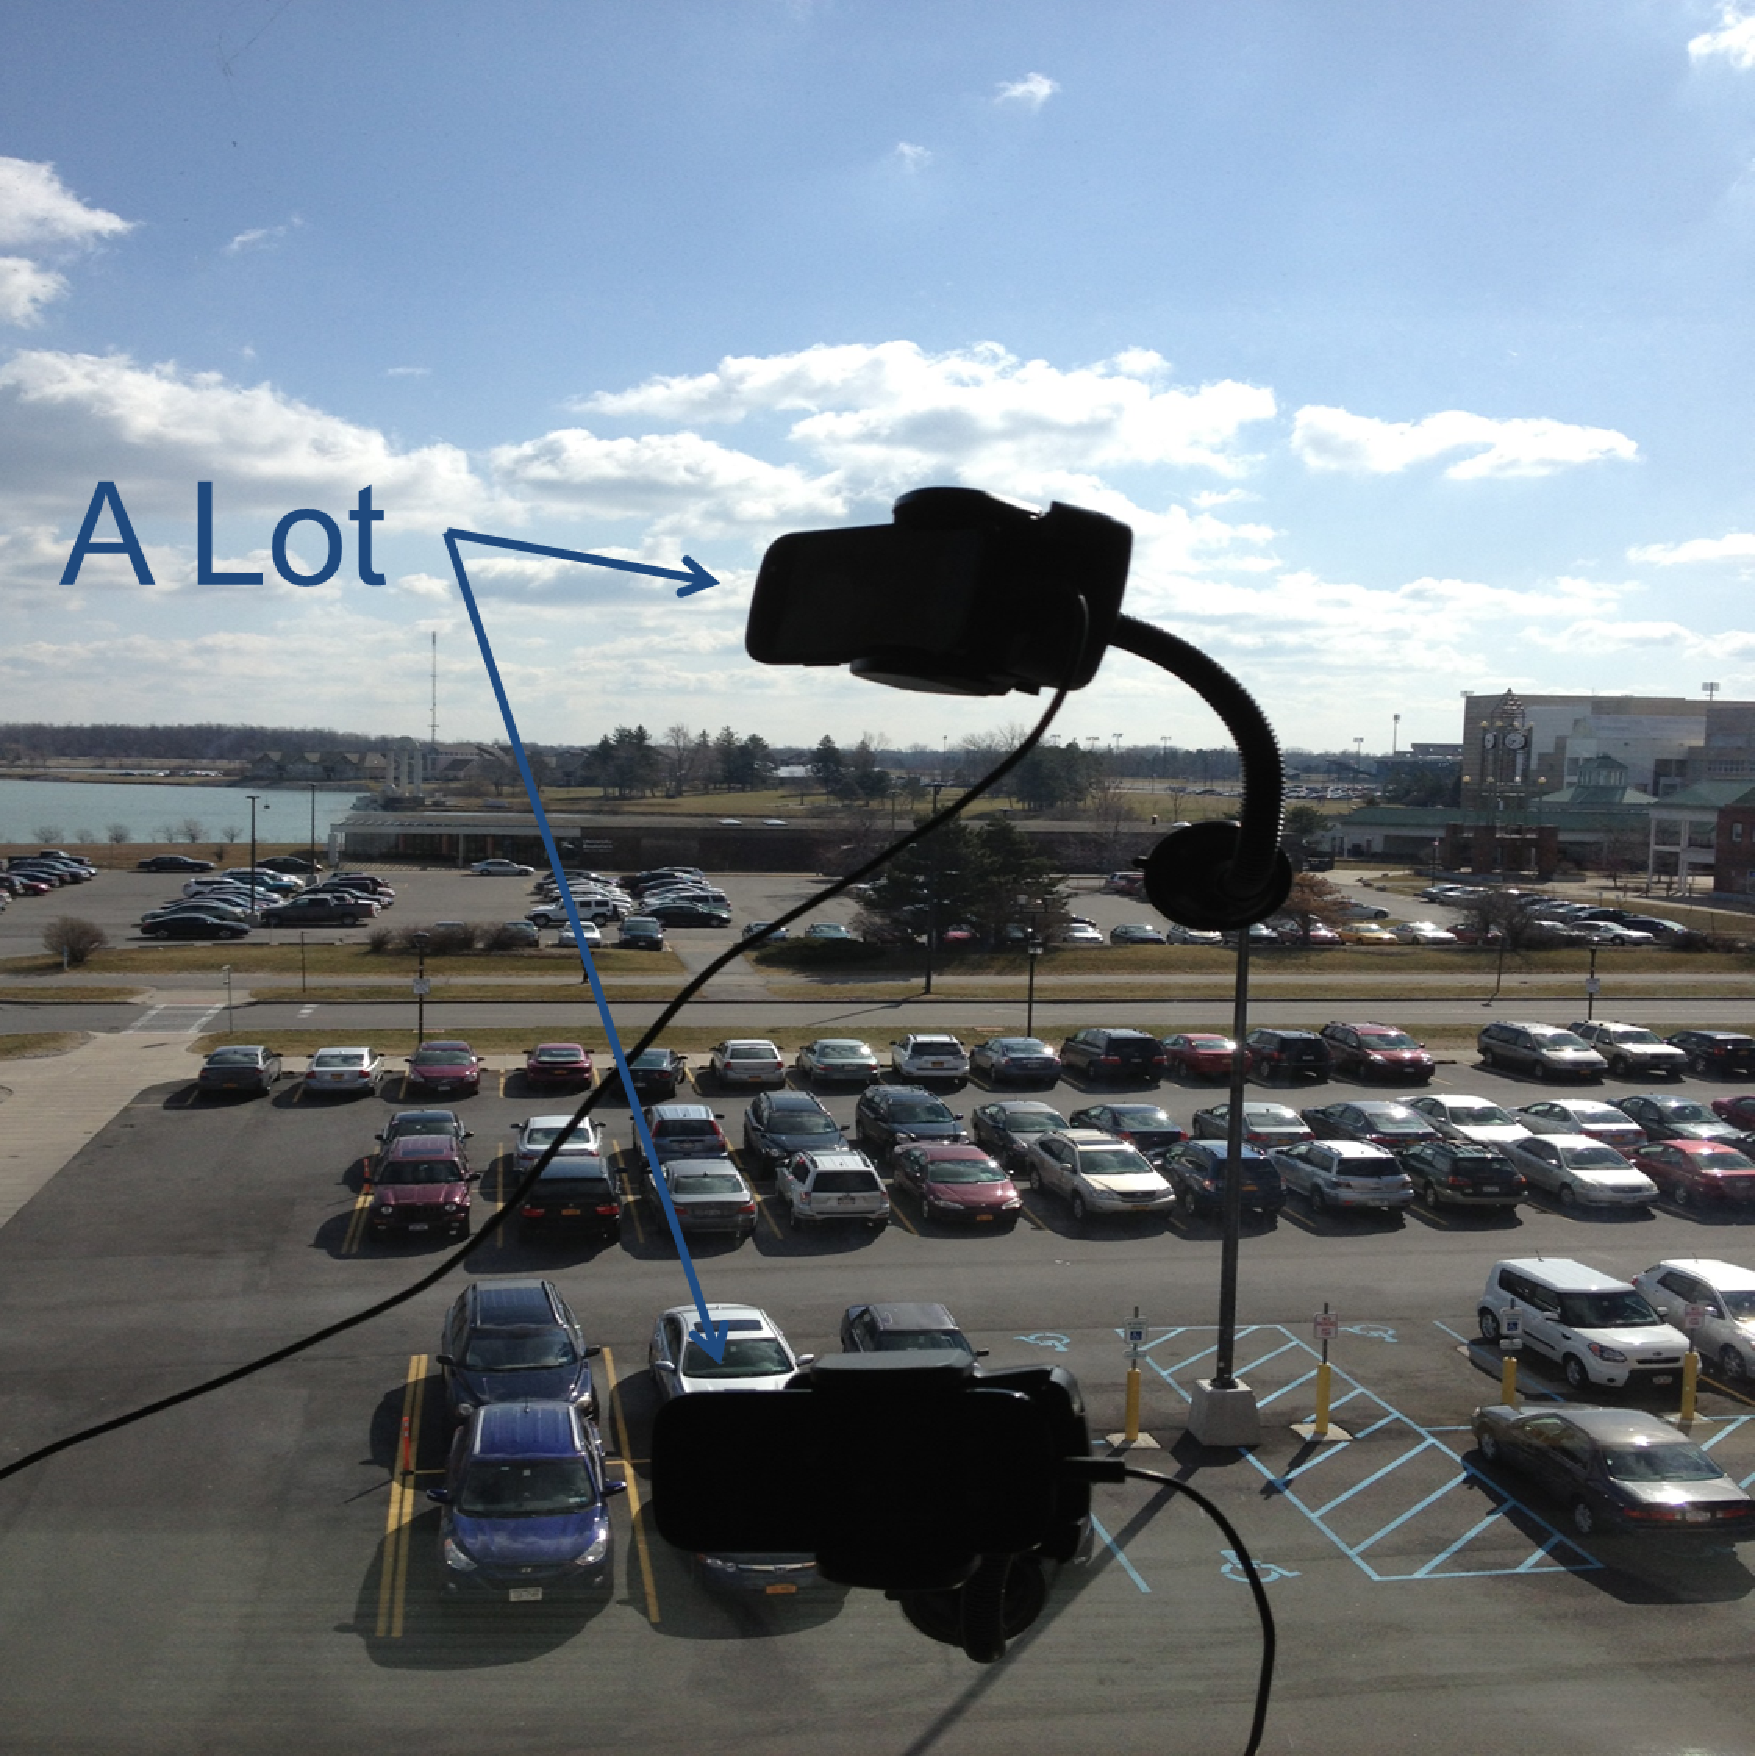
\includegraphics[width=\columnwidth]{./figures/Camera_setting.pdf}

\caption{\textbf{Monitoring cameras.} A view of one of the monitored parking
lots is shown.}

\label{fig-camera}
\end{figure}

\begin{figure}
\centering
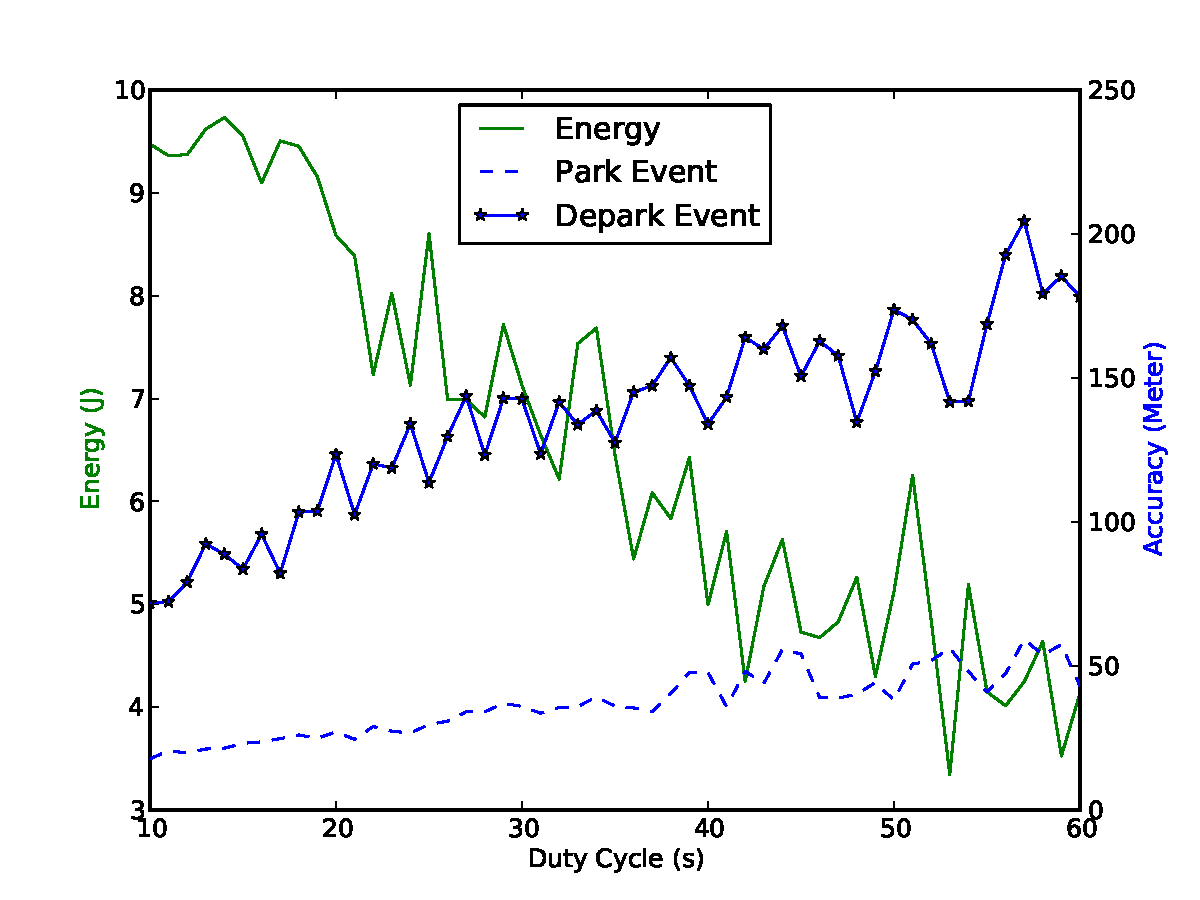
\includegraphics[width=\columnwidth]{./figures/Energy_accuracy.pdf}

\caption{\textbf{Power usage vs. detector accuracy.} \XXXnote{GWA: TODO.}}

\label{fig-energy}
\end{figure}

To furnish further ground truth, we conducted a structured experiment on
\XXXnote{Anand: Add date.}.  Seven volunteers participated, including six men
and one woman, six of whom were right-handed and one of whom was left-handed.
Each was asked to conduct the same experiment:  carrying a mobile phone, walk
out to his car, drive around briefly, park and walk back inside.  Each
participant was further instructed to repeat this experiment ten times,
following set directions as to where to hold or carry the phone while walking
and driving.  Participants spent approximately three to five minutes per run
for a total of slightly under an hour total for the entire experiment.

The experiment permitted us to obtain sensing data from a cross section of
people posessed of varying body morphologies and different habits of driving
cars and handling mobile devices.

\begin{figure*}
\centering
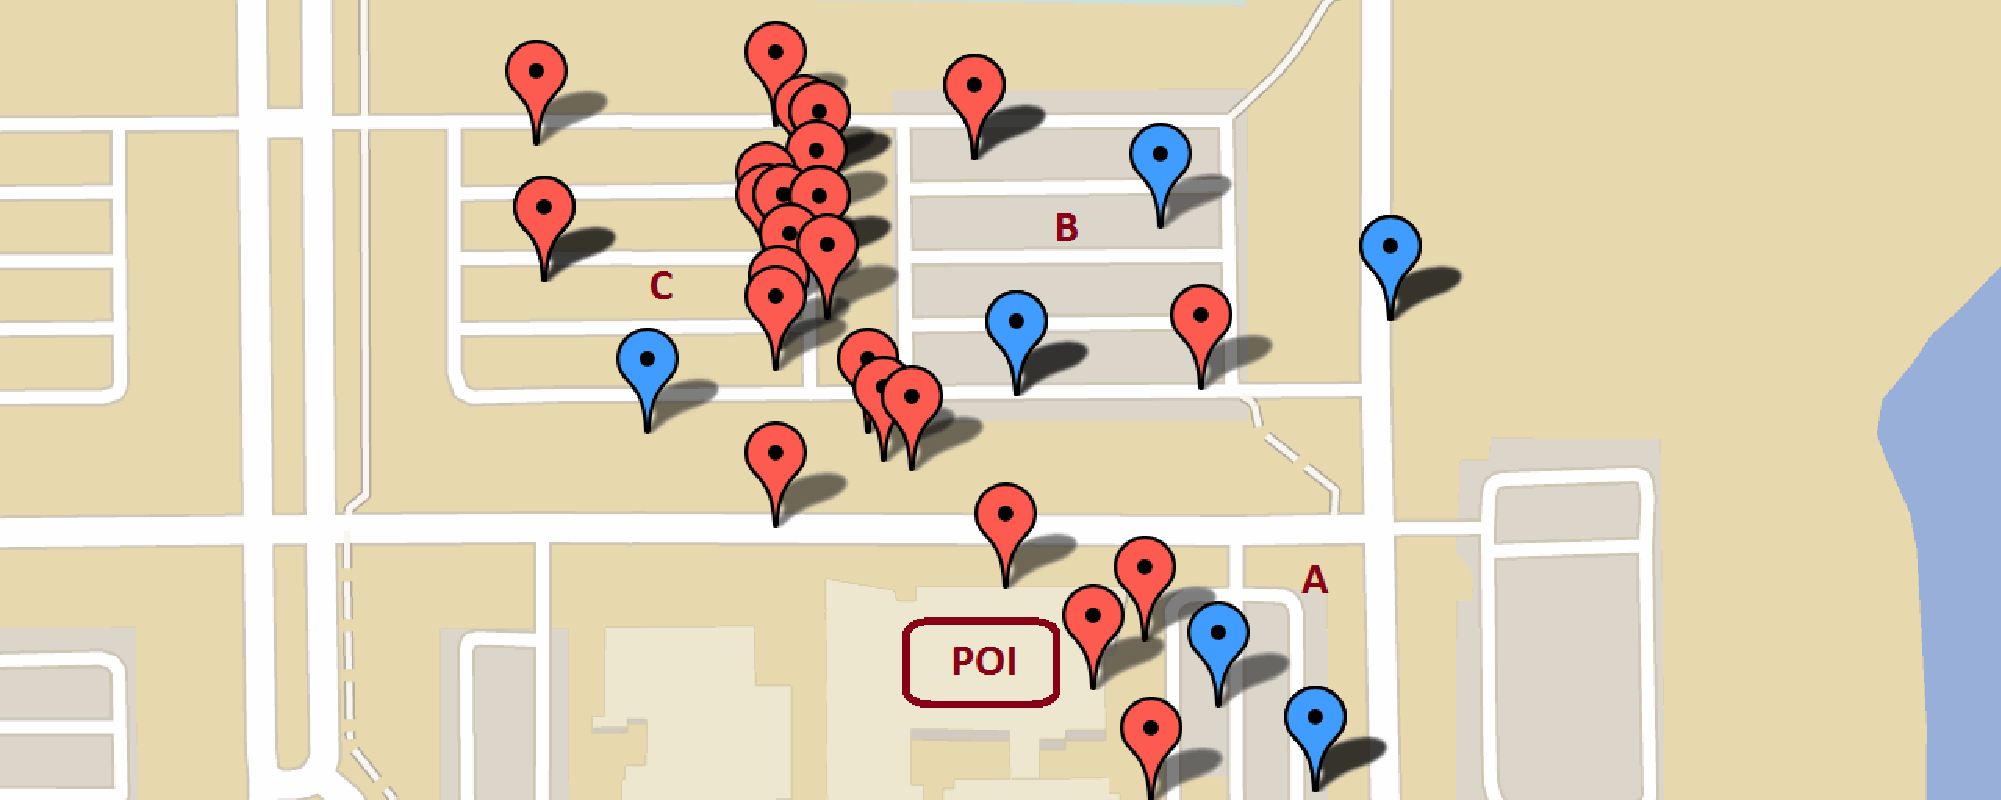
\includegraphics[width=\textwidth,height=2in]{./figures/detectedEventsOnMap.pdf}

\caption{\textbf{Map showing all events detected by PocketParker during our
deployment.} \XXXnote{GWA: TODO.}}

\label{fig-energy}
\end{figure*}

\begin{figure*}
\centering
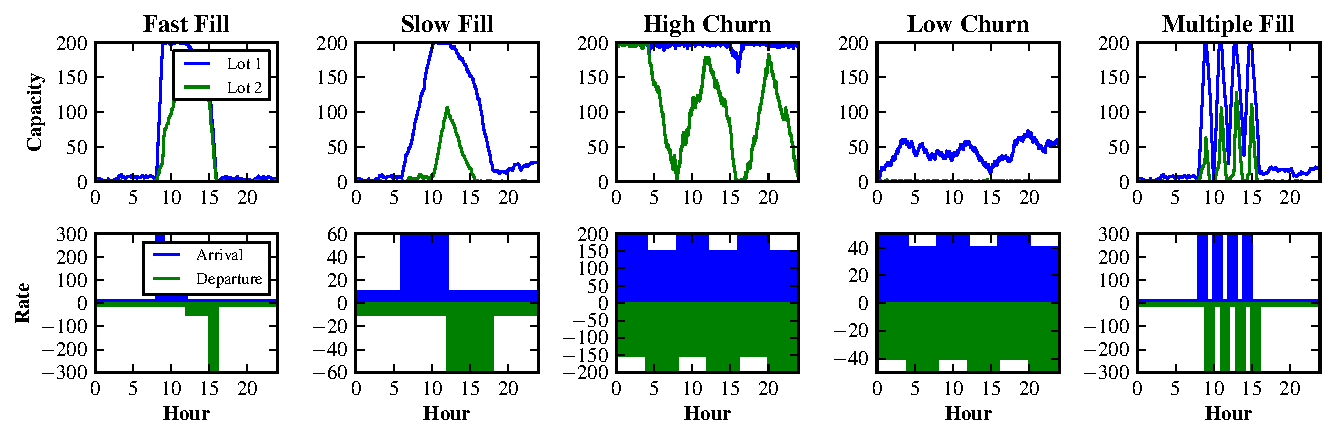
\includegraphics[width=\textwidth]{./simulator/figures/lots.pdf}

\caption{\textbf{Description of each type of lot simulated.} \XXXnote{GWA:
TODO.}}

\label{fig-lotsdescription}
\end{figure*}

\begin{figure*}
\centering
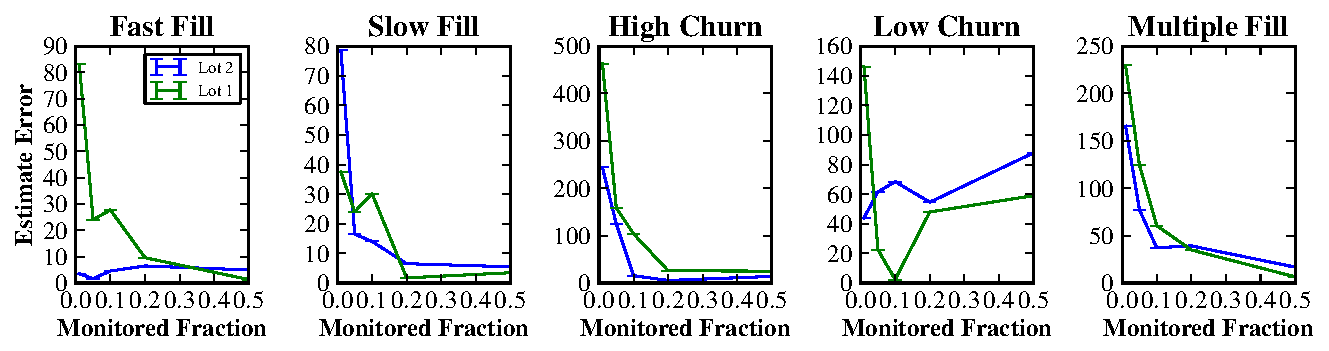
\includegraphics[width=\textwidth]{./simulator/figures/capacity_experiment.pdf}

\caption{\textbf{Errors in capacity estimation.} \XXXnote{GWA: TODO.}}

\label{fig-lotsdescription}
\end{figure*}

